\documentclass[hyperref={pdfpagelabels=false}]{beamer}
\usepackage{graphicx,lmodern,subfigure,ulem,color,graphicx,tikz,booktabs,natbib}
\usepackage{mathrsfs}
\usetheme{Warsaw}
%\definecolor{beamer@blendedblue}{rgb}{0.1,0.5,0.1}
%\definecolor{ForestGreen}{RGB}{60, 140, 60}
%\setbeamercolor{structure}{fg=beamer@blendedblue}
\setbeamertemplate{navigation symbols}{}
\setbeamertemplate{footline}[frame number]
\bibliographystyle{chicago}
\newcommand{\spitem}{\vspace{.3cm}\item}
\newcommand{\elas}{$E_{labor}$}
%\def \FigPath {Users\th3\Documents\Job_Market_Paper\Code\Figures} 


\title{Uncertainty Shocks}
\author{Marco Brianti}
\institute{Boston College}
\date{September 2018}


\begin{document}
	
	\frame{\titlepage \begin{center} Dissertation Workshop \end{center} }
	
	
		\frame{\frametitle{Two Possible Avenues}
		
		
		\begin{enumerate}
			\item News-noise driven uncertainty
			
			\
			
			\item Financial Shocks vs Uncertainty Shocks
		\end{enumerate}
		
		
	}

\frame{\frametitle{Credit Conditions and Uncertainty (I)}


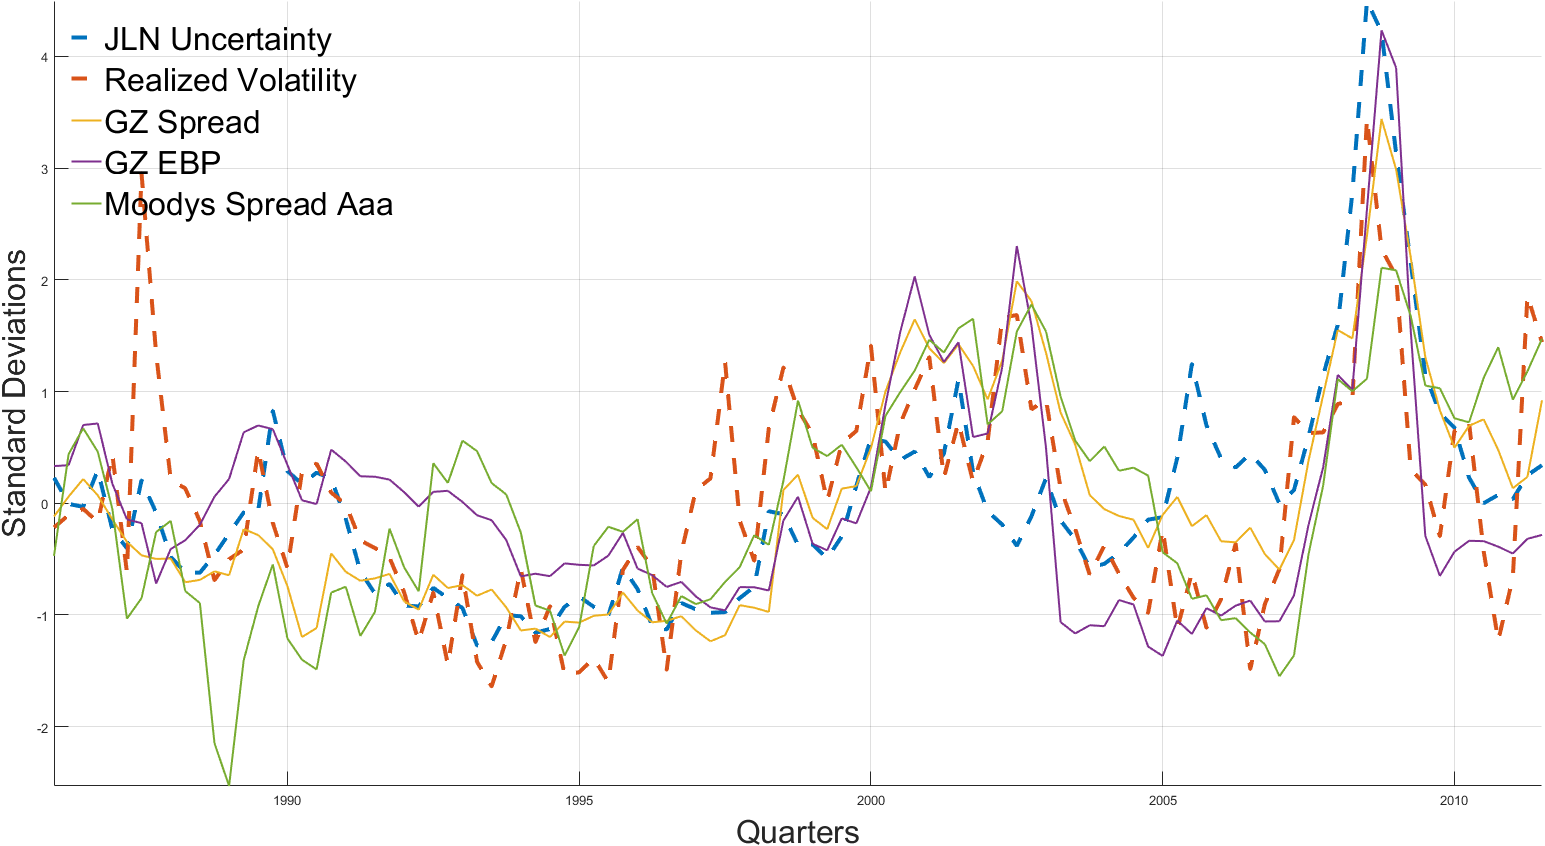
\includegraphics[scale=0.26]{Financial_Uncertainty}

\

Proxies for \textbf{credit conditions} and \textbf{uncertainty} are both countercyclical and tightly correlated.

}


\frame{\frametitle{Credit Conditions and Uncertainty (II)}
	
	
	\begin{table}
		\begin{tabular}{c||cccccc}
            & JLN         &      RV    & GZ  & EBP &    Moodys Aaa 	  \\
            \hline
            \hline
JLN	        &    1        &       -    &      -     &       -    &    -   \\
RV        	&    0.5865   &  1         &     -      &     -      &    -   \\ 
GZ       	&    0.7742   &  0.6247    &  1         &     -      &     -  \\
EBP      	&    0.6213   &  0.5621    &  0.7316    &  1         &     -  \\
Moodys Aaa	&    0.4386   &  0.4554    &  0.7993    &  0.5243    &    1   \\
	\end{tabular}
	\end{table}

\

\

As suggested by the graph above, all the variables are strongly correlated.

}


\frame{\frametitle{Financial Shocks and Uncertainty Shocks}
	
	Stock and Watson (2012); Caldara et al. (2016) among others shown that uncertainty shocks and financial shocks are deeply confounded.
	
	\
	
	\
	
	
	$$
	corr(\iota^{EBP}_t,\iota^{JLN}_t) \approx 0.45
	$$
	
	\
	
	\
	
	
	where $\iota^{EBP}_t$ is an unpredictable innovation in the \textbf{excess bond premium} from Gilchrist and Zakrajzek (2012) and $\iota^{JLN}_t$ is an unpredictable innovation in the \textbf{uncertainty proxy} from Jurado et al. (2015).
	

	

	
	
	
}

\frame{\frametitle{Both a theoretical and empirical question}

	Literature did not succeed yet to disentangle the two exogenous sources for two main reasons:
\begin{enumerate}
	\item Simultaneity
	\begin{itemize}
		\item Both types of variables are fast moving
				\end{itemize}	
			\item Observationally equivalence
			
			\begin{itemize}
			\item They have the same qualitative effects on prices and quantities
\end{itemize}
\end{enumerate}

\

\

As a result, both \textbf{zero-impact restrictions} cannot be used and \textbf{internal instruments} are not available.
	
}

\frame{\frametitle{My contribution}
	
	I want to take a step back and show evidence and theory that financial and uncertainty shocks
	
	
	\begin{itemize}
		
		\item are not observationally equivalent, and
	
		
		\item they can be successfully disentangled.
		
		\end{itemize}
	
	\	
	
	\
	
	
	In particular, I will show evidence that there exists a set of variables which respond differently to financial and uncertainty shocks. 
	\begin{itemize}
		\item there exists an \textbf{economic intuition} for this response
		\item those variables can be used as \textbf{internal instruments}
	\end{itemize}
}
	
		\frame{\frametitle{Variables of Interest}
		

\textbf{Cash Flow} is defined as (i) undistributed corporate profits plus (ii) consumption of fixed capital minus (iii) net capital transfers paid.

\

where 

\begin{enumerate}
	\item \textbf{Undistributed corporate profits} are defined as (i) corporate profits minus (ii) dividends
	\item \textbf{consumption of fixed capital} can be simply interpreted as capital depreciation
	\item \textbf{net capital transfers paid} are unrequited transfers, e.g. charity
\end{enumerate}

\

\textbf{Cash Flow} is a profit-related measure of \textbf{internal funds} available for investment. [The NIPA Handbook, December 2015]

	}


\frame{\frametitle{Partial Equilibrium Analysis (I)}
	
	Decrease in the risk bearing capacity of the financial sector. 
	
	\begin{figure}[plain]
		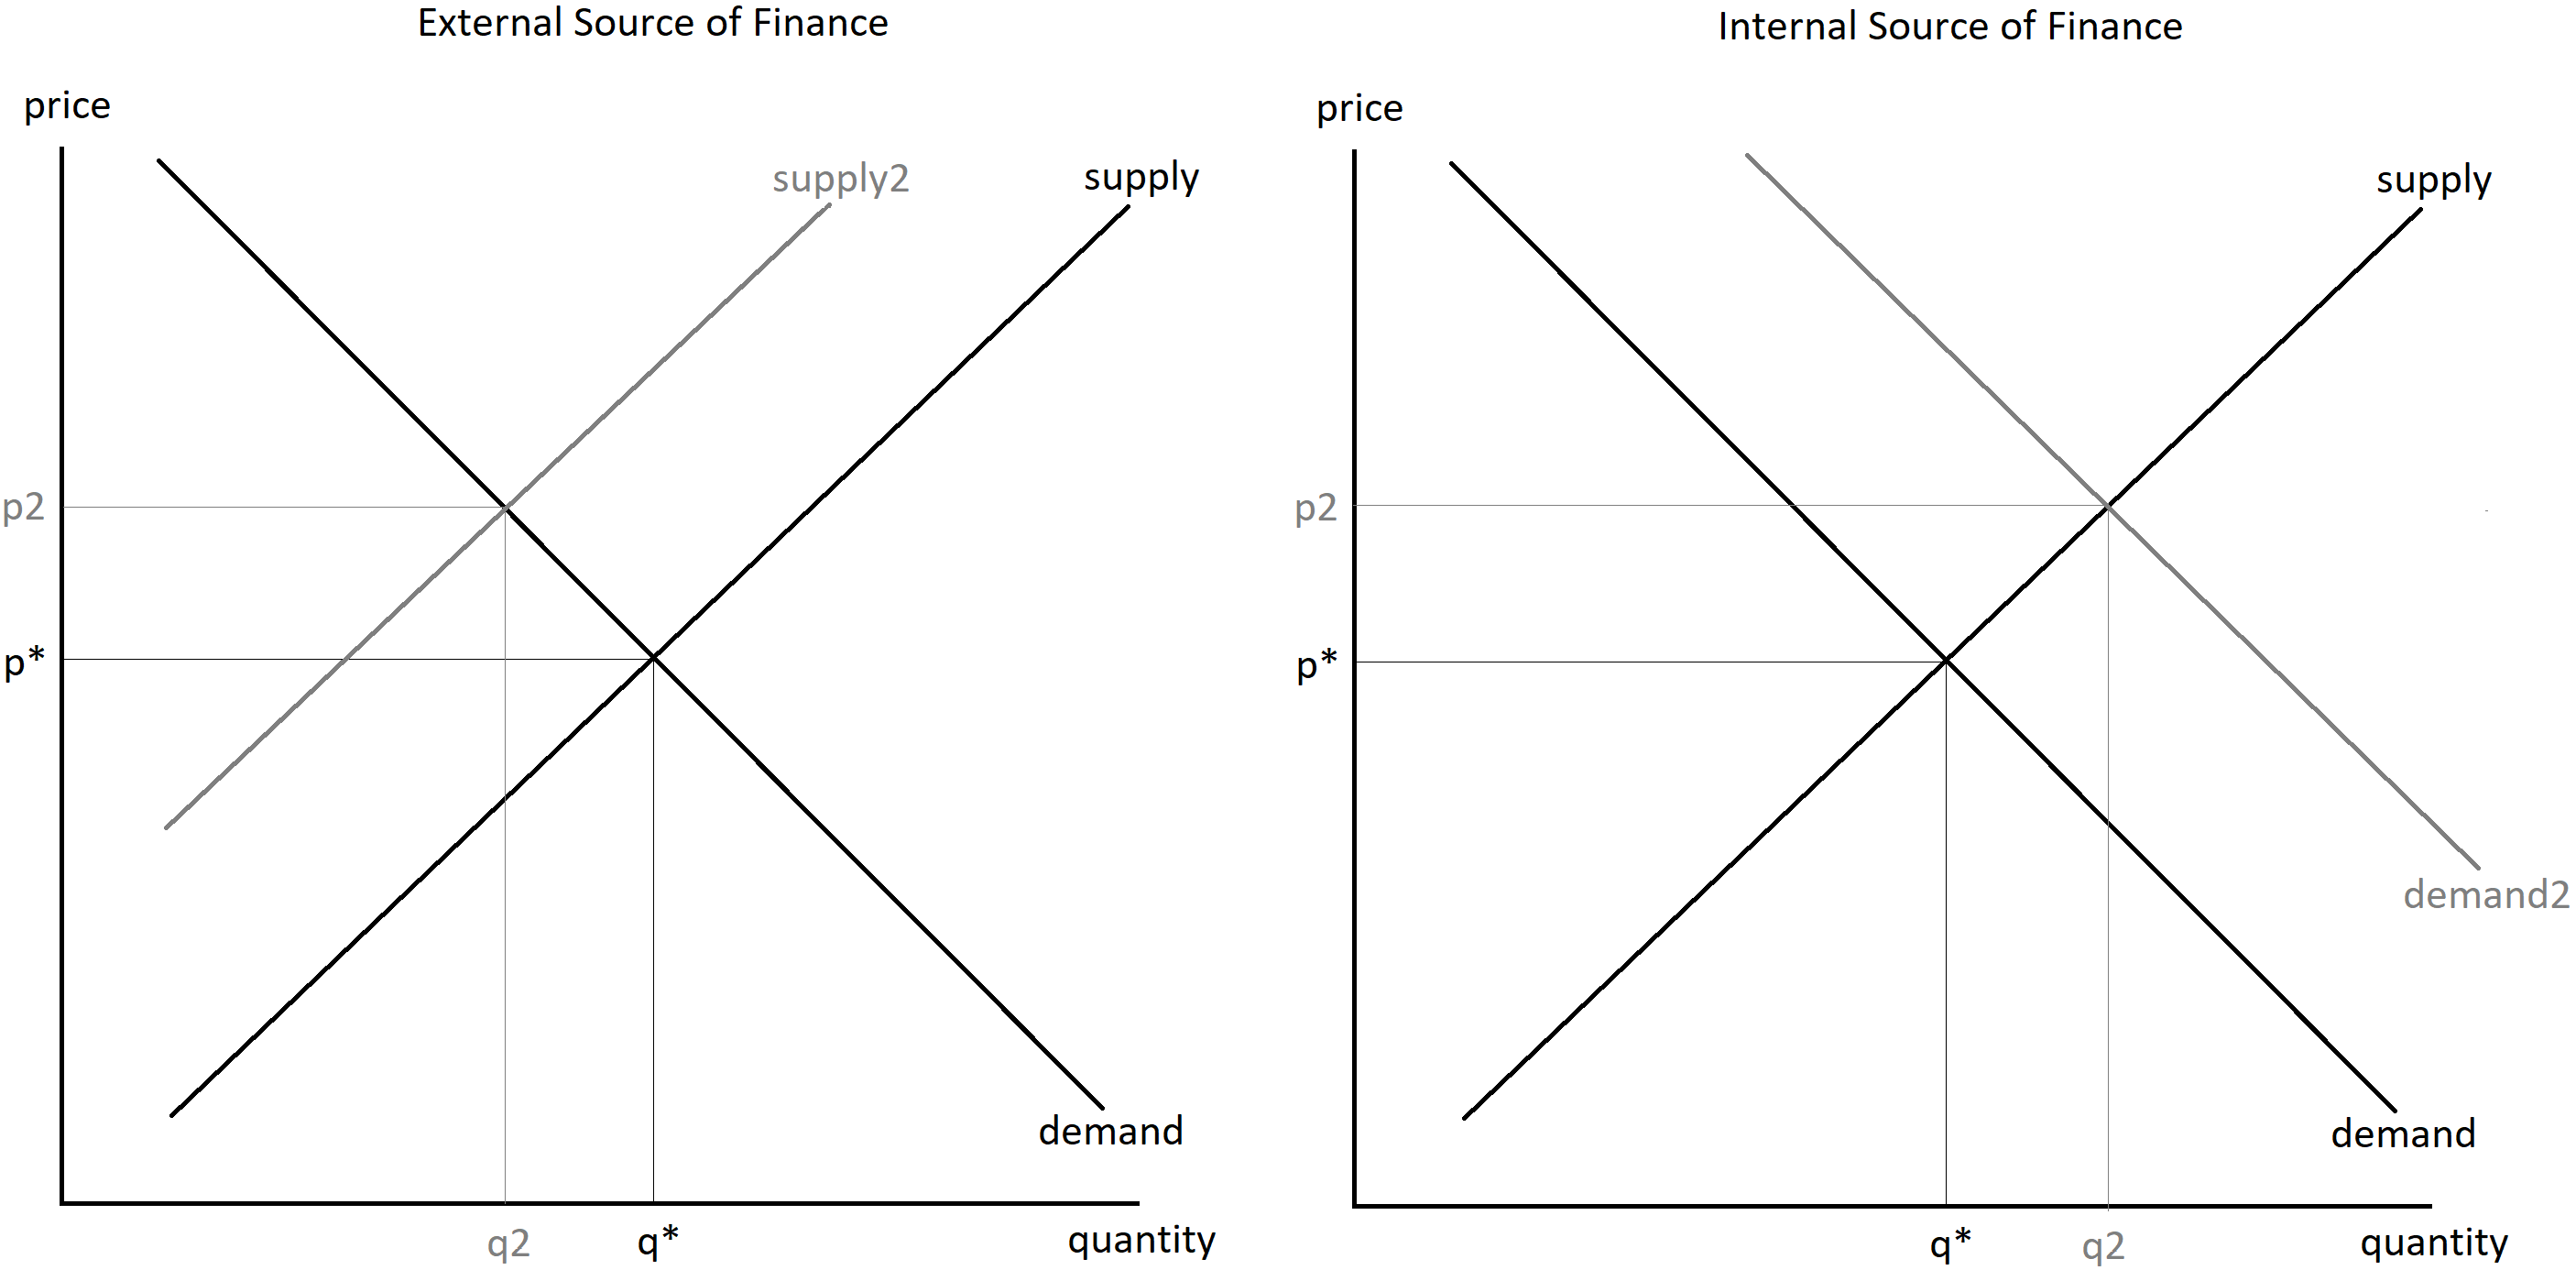
\includegraphics[scale=0.13]{fig_financial_supply_demand_F}
	\end{figure}
	
	Notice that I am taking as given the supply of internal source of finance. 
}

\frame{\frametitle{Partial Equilibrium Analysis (II)}
	
	Increase in the level of uncertainty. 
	
	\begin{figure}[plain]
		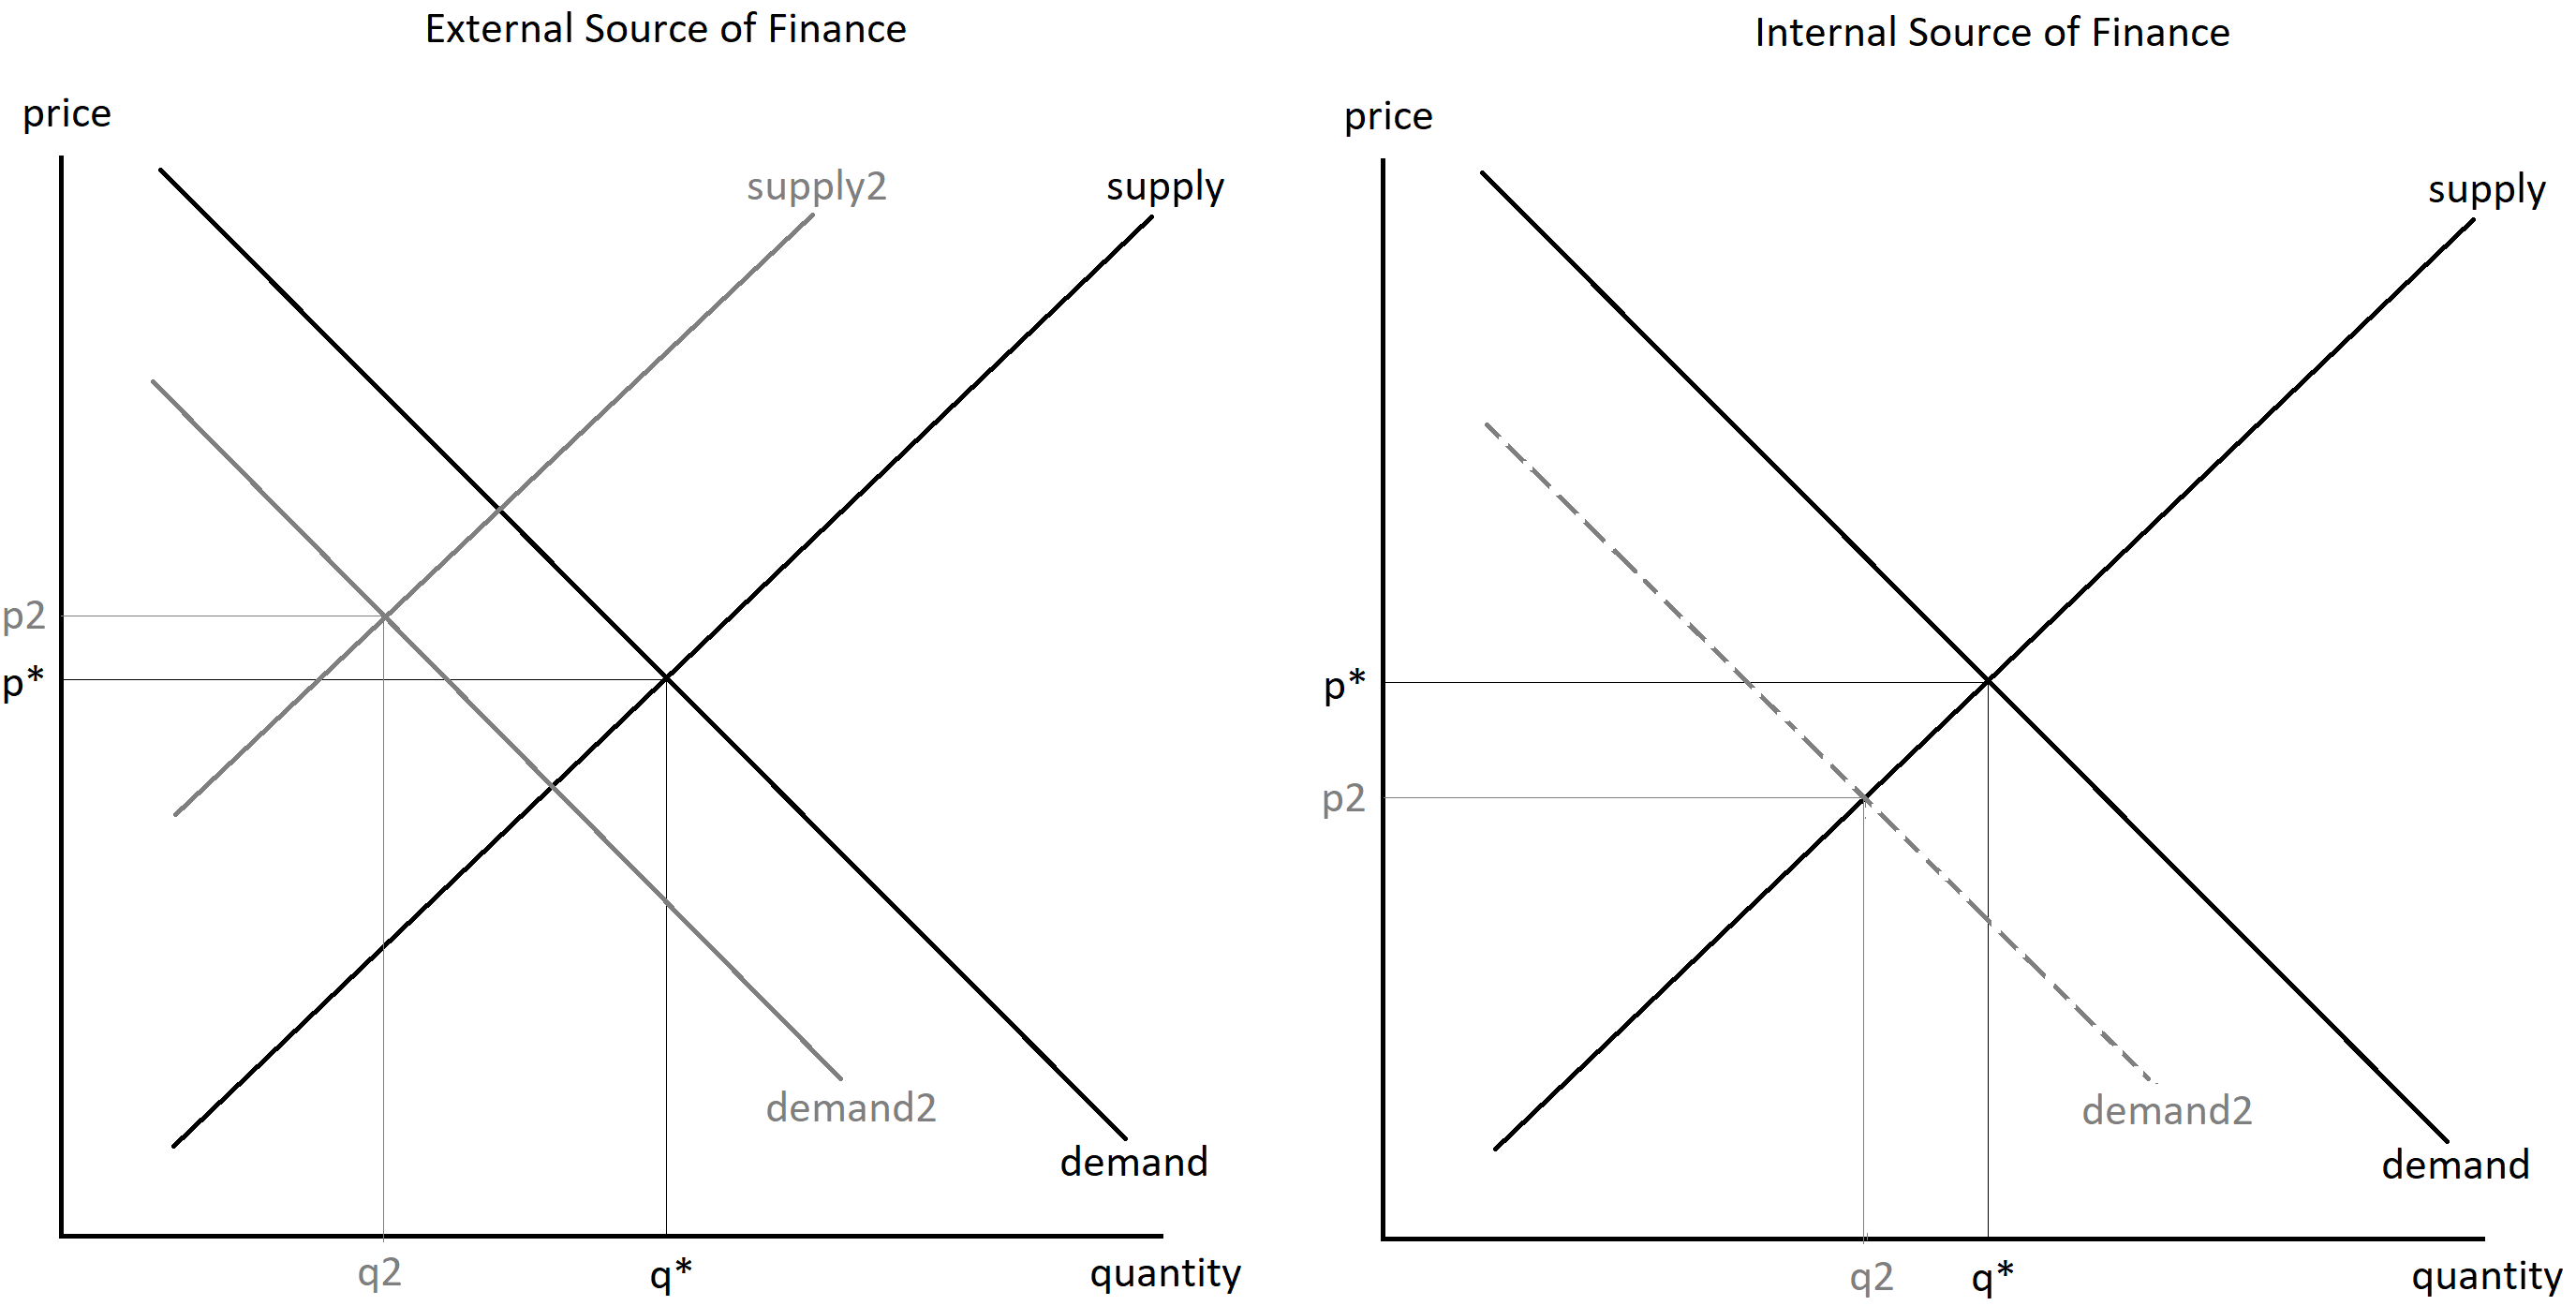
\includegraphics[scale=0.13]{fig_financial_supply_demand_U}
	\end{figure}
	
	Notice that I am taking as given the supply of internal source of finance. 
	
}


\frame{\frametitle{Economic Intuition}
	
	
	\begin{itemize}
		
		\item 	After a \textbf{decrease in credit supply}, quantity of the internal source of finance should increase.
		
		\begin{itemize}
			\item Controlling for supply of internal funds cash flow should increase.
		\end{itemize}
		
		\
		
		\
		
		\item After an \textbf{increase in uncertainty}, quantity of the internal source of finance should either decrease or remain unchanged.
		
	\begin{itemize}
	\item Controlling for supply of internal funds cash flow should either decrease or remain unchanged.
\end{itemize}
		
		
		
		
	\end{itemize}
	
}	
	
	\frame{\frametitle{Controlling for the Supply of Internal Funds}	
		
		The main source of internal funds available for investment is the \textbf{flow profit} of the current year.
		
		\
		
		In order to control for general equilibrium effect, cash flow needs to be normalized by the corporate profit.
		
		In particular, normalized cash flow can be thought as an index between $0$ and $1$
		\begin{itemize}
			\item If the index is equal to zero, current profits are fully distributed outside the firm
			\item If index is equal to one, current profits are going to be internally used
		\end{itemize}
	
	
	
	
	

		
	}
	

\frame{\frametitle{Suggestive Evidence}
	
	Run the following regression,
	
	\
	
	$$
	\frac{CF_t}{CP_t} = \alpha + B(L)X_{t-1} + \beta^{F} F_t + \beta^{U} U_t + \varepsilon_t
	$$
	
	\
	
	where $CF_t$ and $CP_t$ are cash flow and corporate profits as described above, $X_{t-1}$ is a vector of control variables,
	
	\
	
	$$
	X_{t-1} = [GDP_{t-1} \ I_{t-1} \ C_{t-1} \ SP_{t-1} \ H_{t-1} \ U_{t-1} \ F_{t-1} \ CF_{t-1}/CP_{t-1}]
	$$
	
	\
	
	and $F_t$ and $U_t$ are proxies for financial conditions and uncertainty levels, respectively. 

	
}

	
	\frame{\frametitle{Results}
		

Benchmark regression,
$$
\frac{CF_t}{CP_t} = \alpha + B(L)X_{t-1} + \beta^{F} F_t + \beta^{U} U_t + \varepsilon_t
$$

\

\

\begin{itemize}
	\item $\beta^F$ is always positive and significant at $1$\%.
	
	\
	
	\
	
	\item $\beta^U$ is either negative and significant at $10$\% or not significant. 
\end{itemize}

			





		
	}



	

	\frame{\frametitle{Technically Speaking (I)}
		
		Assume you use OLS techniques to regress $X_t$ on its own past
		$$
		X_t = B_1 X_{t-1} + B_2 X_{t-2} + \dots + B_p X_{t-p} + \iota_t
		$$
		where $X_t = [U_t \ \  Y_t  \ \  F_t]'$, $U_t$ represents a proxy for uncertainty, $Y_t$ a column vector of macro variables, and $F_t$ a vector of financial variables.
		
		\
		
		Moreover, $\iota_t = [\iota^U_t \ \ \iota^Y_t \ \ \iota^F_t]'$ is a vector of time-varying innovations related to the corresponding variables.
		
		\
		
		In general, $\iota_t$ does not represent a vector of structural shocks since 
		$$
		\iota_t \iota_t' \neq I_n
		$$
		which implies that innovations represent a (linear) combination of the structural shocks.
	}

	\frame{\frametitle{Technically Speaking (II)}
	
	
	Structural VARs methods aim to solve the following system in order to recover structural shocks
	$$
	\iota_t = C s_t \ \ \Rightarrow \ \ s_t = C^{-1} \iota_t \ \ \Rightarrow \ \ s_t = A \iota_t
	$$
	which is
	$$
    \begin{cases}
	s_t^U = A_{11} \iota_t^U + A_{12} \iota_t^Y + A_{13} \iota_t^F \\
	s_t^Y = A_{21} \iota_t^U + A_{22} \iota_t^Y + A_{23} \iota_t^F \\
	s_t^U = A_{31} \iota_t^U + A_{32} \iota_t^Y + A_{33} \iota_t^F
	\end{cases}
$$

\begin{enumerate}
	\item \textbf{Latent variable} $\Rightarrow$ $\iota_t^U$ may not represent innovations to uncertainty
	
	
	\item \textbf{Simultaneity} $\Rightarrow$ Each element of $A$ is different from zero
	
	\item \textbf{Reverse causality} $\Rightarrow$ $\iota_t^U$ may be lead by $s_{t,t+h}$, $h > 0$
	
	
	\item \textbf{Financial shocks} $\Rightarrow$ $E [ \iota_t^U  \iota_t^{F'}]  \neq 0$ and large
	
\end{enumerate}

}


	\frame{\frametitle{(1) Latent Variable}
		
		Not surprisingly, $Corr(VXO_t, JLN_t) = 0.4139$
		
		\
		
		However, $Corr(\iota_t^{VXO},\iota_t^{JLN}) \in [-0.1865 \ \ 0]$
	
\

Which means that although the 2 raw series are highly correlated, once we control for available information at $t-1$ then they convey different information.

\

\textbf{Solution.} JLN proxy is consistent with the theoretical definition of uncertainty. 

\

$\Rightarrow$ VXO measures \textbf{macro volatility} and not macro uncertainty.

	
}




	\frame{\frametitle{(2) Simultaneity with other shocks}

	
In general,	
$$
corr(\iota^{JLN}_t,s^Y_t) \approx 0
$$
which implies that uncertainty innovations are fairly uncorrelated with macro structural shocks series derived in the literature.

\

$s_t^Y$ are several series of macro structural shocks derived by the literature (possibly via narrative approach). 
\begin{itemize}
	\item Romer and Romer (2010) unanticipated tax shocks
	\item Martens and Ravn (2011) labor productivity shocks
	\item Leeper et al. (2013) anticipated tax shocks
	\item Kilian (2009) oil shocks
	\item \dots
\end{itemize}
}


	\frame{\frametitle{(3) Reverse causality with news shocks}
		
		\begin{itemize}
			
			\item \textbf{JLN proxy} controls for the forecastable part of each variable
			
			\
			
			
			\item Some structural shocks shown above are \textbf{anticipated}
			
			\
			
			
			\item We can possibly control for \textbf{news shocks} to TFP
			\begin{itemize}
				\item However, we will have to assume that TFP is fully exogenous
			\end{itemize}
			
			\
			
			
			\item \textbf{Surveys} can help for the short run horizon
			\begin{itemize}
				\item SPF has the best timing
			\end{itemize}
		
		\
		
		
			\item Most importantly, we should control for the shocks and the \textbf{square of the shocks}
			\begin{itemize}
				\item Potentially, uncertainty may evenly react for large shocks no matter the sign
			\end{itemize}
		
		
		\end{itemize}
	
}

	\frame{\frametitle{(4) Financial Shocks vs Uncertainty Shocks}
	
Stock and Watson (2012); Caldara, Fuentes-Albero, Gilchrist, and Zakrajzek (2016) shown that uncertainty shocks and financial shocks are deeply confounded.
$$
corr(\iota^{EBP}_t,\iota^{JLN}_t) \approx 0.45
$$
where $\iota^{EBP}_t$ is an innovation in the \textbf{excess bond premium} from Gilchrist and Zakrajzek (2012).

\

\

Literature did not succeed yet to disentangle the two exogenous sources:
\begin{itemize}
	\item \textbf{External instruments} do not seem to be available
	\item \textbf{Internal instruments} are difficult to find because variables respond analogously to both shocks
\end{itemize}
	
}



	\frame{\frametitle{(4) Financial Shocks vs Uncertainty Shocks - Solution (I)}
		
I propose a \textbf{novel family of internal instruments} which can help out to disentangle the two exogenous shocks.	

\

\textbf{Economic Intuition.} 

\begin{itemize}
	\item An exogenous deterioration of credit conditions should display the attempt of borrowers to fund their projects with \textbf{alternative sources} (at least on impact): internal cash flow, equity issuance, ...
	\item Alternatively, following real-options models (Bernanke, 1983; Brennan and Schwartz, 1985; McDonald and Siegel, 1986) after an uncertainty shock firms prefer to \textbf{wait-and-see} without undertake any investment.
\end{itemize}

	
	}


	\frame{\frametitle{(4) Financial Shocks vs Uncertainty Shocks - Solution (II)}
	
	Although the impact effect on investment is expected to be negative in both cases, I expect
	\begin{itemize}
		\item a financial shock to have a \textbf{negative impact} on internal cash flow;
		\item an uncertainty shock to have a \textbf{non-negative impact} on internal cash flow.
	\end{itemize}

\

\
	
The two shocks can be disentangled via \textbf{sign restrictions} \`a la Uhlig (2005)
	
	
}


\end{document}